%==========================================================
\section{Préemption et ordonnancement}
%==========================================================

% --- Our library vs pthreads with taskset ---
\begin{frame}{Notre bibliothèque vs \texttt{pthreads} sous \texttt{taskset}}
  \vfill
  \begin{center}
      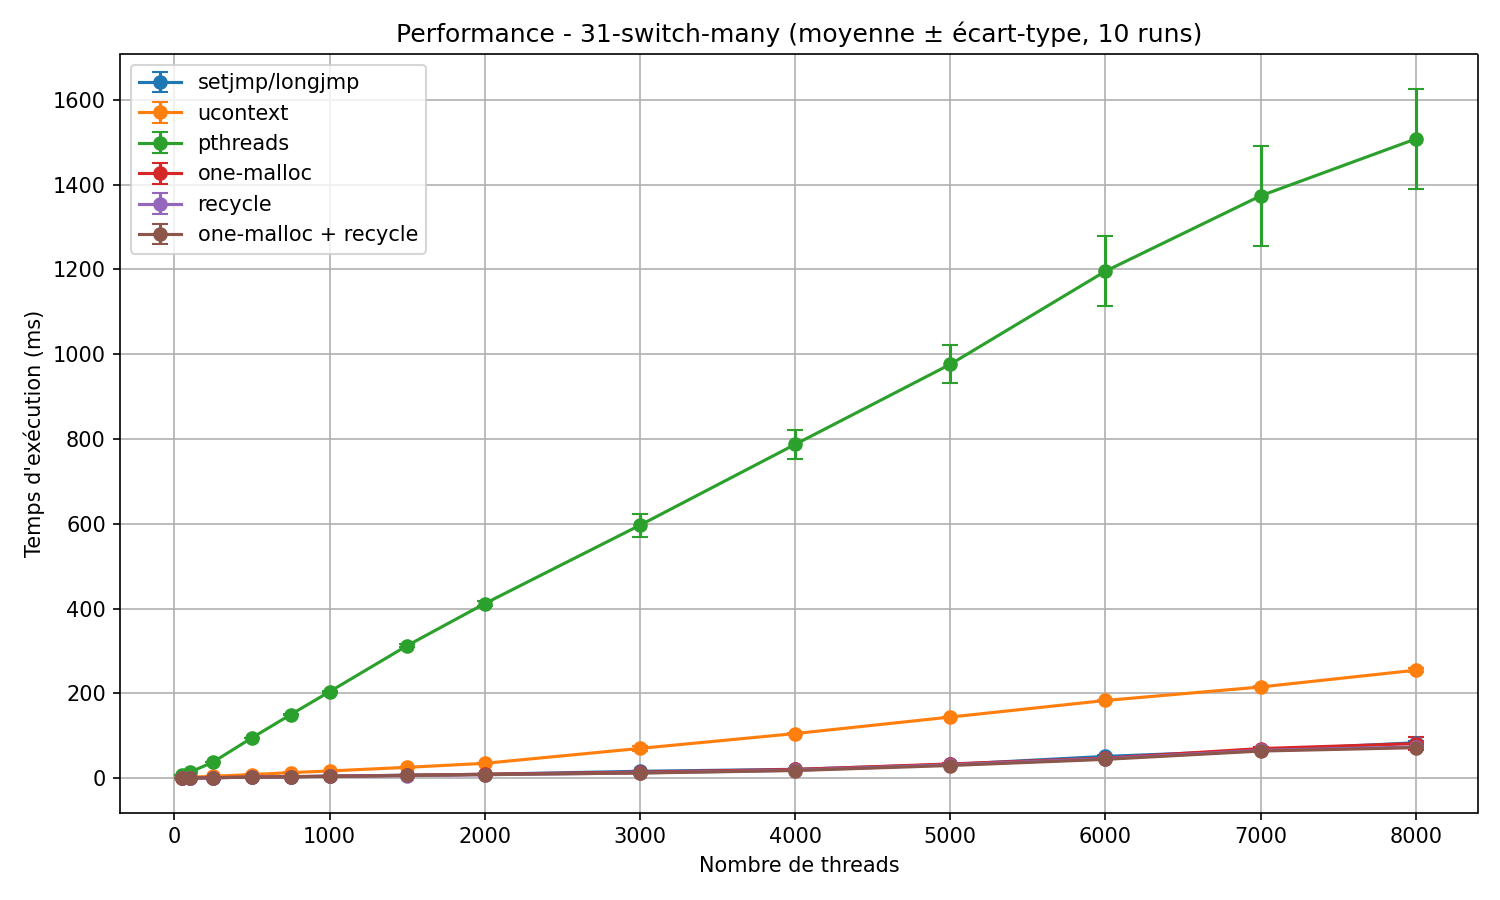
\includegraphics[width=0.78\linewidth]{rapport-final/images/31-switch-many-pthread.png}
  \end{center}
  \vfill
\end{frame}

% --- Our library vs pthreads without taskset ---
\begin{frame}{Notre bibliothèque vs \texttt{pthreads} sans \texttt{taskset}}
  \vfill
  \begin{center}
      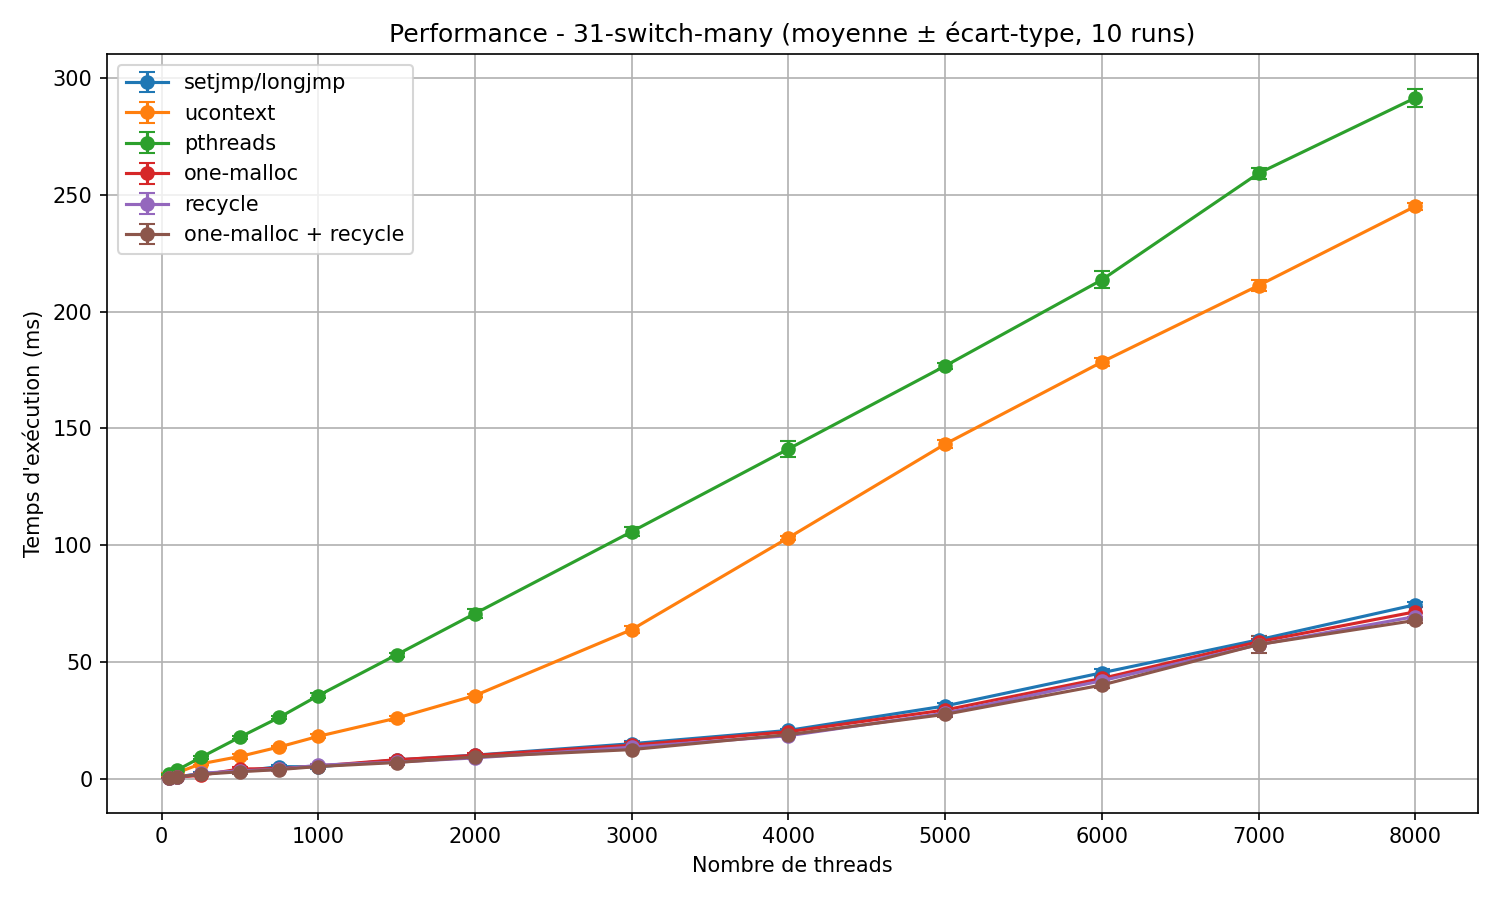
\includegraphics[width=0.78\linewidth]{rapport-final/images/31-switch-many-no-taskset.png}
  \end{center}
  \vfill
\end{frame}


%=================================================
% PREEMPTION 1
%=================================================

\begin{frame}{Préemption : principe et fonctionnement}

\begin{columns}

\column{0.52\textwidth}

\textbf{Objectif :}
\begin{itemize}
    \item Interrompre automatiquement un thread
    \item Éviter qu'un thread monopolise le CPU
\end{itemize}

\vspace{0.3cm}

\column{0.45\textwidth}

\begin{center}
\begin{tikzpicture}[
    node distance=1.4cm,
    every node/.style={font=\small},
    box/.style={
        draw,
        rounded corners,
        minimum width=2.8cm,
        minimum height=0.9cm,
        align=center
    }
]

\node[box, fill=blue!15] (timer) {Timer\\\texttt{setitimer()}};

\node[box, fill=orange!20, below of=timer] (sig) {Signal\\\texttt{SIGVTALRM}};

\node[box, fill=green!20, below of=sig] (handler) {Handler};

\node[box, fill=red!20, below of=handler] {\texttt{thread\_yield()}};

\draw[-{Latex[length=2mm]}] (timer) -- (sig);
\draw[-{Latex[length=2mm]}] (sig) -- (handler);
\draw[-{Latex[length=2mm]}] (handler) -- ++(0,-0.6);

\end{tikzpicture}
\end{center}

\end{columns}

\end{frame}

%=================================================
% PREEMPTION 2
%=================================================

\begin{frame}[fragile]{Protection des sections critiques}

\textbf{Problème :}

\vspace{0.2cm}

Une interruption pendant une modification du scheduler peut :
\begin{itemize}
    \item corrompre les listes chaînées
    \item perdre des threads
    \item provoquer un comportement incohérent
\end{itemize}

\begin{columns}

\column{0.4\textwidth}

\begin{block}{\small Blocage}
\small
\begin{verbatim}
lock_preemption(){
  signals_blocked++;
}
\end{verbatim}
\end{block}

\column{0.4\textwidth}

\begin{block}{\small Réactivation}
\small
\begin{verbatim}
unlock_preemption(){
  signals_blocked--;
}
\end{verbatim}
\end{block}

\end{columns}

\vspace{1cm}

\textbf{\small Structures protégées :} {\small \texttt{readyQueue} / \texttt{blockedQueue} / \texttt{currentThread}}

\end{frame}

%=================================================
% AGING 1
%=================================================

\begin{frame}{Principe du Aging}

\textbf{Objectif :}
\begin{itemize}
    \item Éviter qu’un thread attende trop longtemps
    \item Améliorer l’équité du scheduler
\end{itemize}

\vspace{0.5cm}

\textbf{Principe utilisé :}
\begin{itemize}
    \item Chaque thread possède une priorité
    \item Plus un thread attend dans la \texttt{readyQueue},
    plus sa priorité augmente
\end{itemize}

\vspace{0.6cm}

\begin{center}
\begin{tikzpicture}[
    every node/.style={font=\small}
]

\node[draw, rounded corners, fill=red!20]
(B1) at (0,0) {10};

\node[draw, rounded corners, fill=orange!20]
(B2) at (2.5,0) {7};

\node[draw, rounded corners, fill=yellow!20]
(B3) at (5,0) {3};

\node[draw, rounded corners, fill=green!20]
(B4) at (7.5,0) {1};

\draw[-{Latex[length=2mm]}] (B1) -- (B2);
\draw[-{Latex[length=2mm]}] (B2) -- (B3);
\draw[-{Latex[length=2mm]}] (B3) -- (B4);

\end{tikzpicture}
\end{center}

\vspace{0.4cm}

\begin{block}{Idée clé}
Un thread ancien devient progressivement prioritaire.
\end{block}

\end{frame}



%=================================================
% AGING 2
%=================================================
\begin{frame}[fragile]{Implémentation dans le scheduler}

\textbf{Mise à jour des priorités dans \texttt{thread\_yield()} :}

\vspace{0.3cm}

\begin{block}{Aging des threads en attente}
\small
\begin{verbatim}
TAILQ_FOREACH(it, &readyQueue, entries) {
    if (it->priority > 0) {
        it->priority--;
    }
}
\end{verbatim}
\end{block}

\vspace{0.5cm}

\textbf{Fonctionnement :}
\begin{itemize}
    \item À chaque changement de contexte :
    \begin{itemize}
        \item les threads en attente gagnent en priorité
    \end{itemize}

    \item Le thread exécuté est réinitialisé (priority = 10) :
\end{itemize}

\end{frame}

%=================================================
% AGING 3
%=================================================
\begin{frame}[fragile]{\texttt{enqueue\_ready} : insertion dans la readyQueue}

\textbf{Principe :} la position dépend uniquement de la priorité.

\vspace{0.3cm}

\begin{block}{Code}
\small
\begin{verbatim}
TAILQ_FOREACH(iter, &readyQueue, entries) {
    if (t->priority < iter->priority) {
        TAILQ_INSERT_BEFORE(iter, t, entries);
        return;
    }
}
\end{verbatim}
\end{block}

\end{frame}